% LaTeX-Vorlage Version 3.0,  Juni 2010
% erstellt von Dr. Andreas Drauschke und Dr. Susanne Teschl
% Modifiziert von Dr. Andreas Mehrle (andreas.mehrle@mci.edu)

\documentclass[a4paper,oneside,10pt]{article}
% PDF-kompatible Auswahl aus der vorhandenen MCI-Vorlage (Version 3.0).
\usepackage[T1]{fontenc}
\usepackage{lmodern}
\usepackage[utf8]{inputenc}
\usepackage[ngerman]{babel}
\usepackage{graphicx}
\usepackage[tmargin=1in,bmargin=1in,lmargin=1.25in,rmargin=1.25in]{geometry}
\usepackage{xcolor,float,amsmath,amssymb,array}
\usepackage{url}
\definecolor{MSBlue}{rgb}{.204,.353,.541}
\definecolor{MSLightBlue}{rgb}{.31,.506,.741}
\setlength{\parindent}{0pt}
\setlength{\emergencystretch}{3em}
\setlength{\parskip}{1ex plus .2ex minus .2ex}
\setlength{\headheight}{14pt}
\newcommand{\offen}[1]{\textcolor{MSBlue}{\textbf{Offen:} #1}}



% Layout der gelieferten Vorlage, mit PDF-kompatiblen Paketen.
\usepackage{ifthen}
\newboolean{english}
\renewcommand{\contentsname}{Inhaltsverzeichnis}
\renewcommand{\listfigurename}{Abbildungsverzeichnis}
\renewcommand{\listtablename}{Tabellenverzeichnis}
\makeatletter
\renewcommand{\section}{\@startsection{section}{1}{0pt}{-2.3ex plus -.5ex}{1ex}{\normalfont\Large\bfseries\color{MSBlue}}}
\renewcommand{\subsection}{\@startsection{subsection}{2}{0pt}{-1.8ex plus -.4ex}{.7ex}{\normalfont\large\sffamily\bfseries}}
\newcommand{\formeleintrag}[1]{\addcontentsline{frm}{figure}{\protect\numberline{\theequation}#1}}
\newcommand{\formeleintragalign}[1]{\addcontentsline{frm}{figure}{\protect\numberline{\number\numexpr\value{equation}+1\relax}#1}}
\newcommand{\listofformeln}{\section*{Formelverzeichnis}\@starttoc{frm}}
\makeatother

\def\labtitle{Biosignalverarbeitung}
\def\labcode{MGST-B-3-BB-BS-ILV}
\def\labname{Aufbau der Hardware und Datenakquise}
\def\labnum{1}
\def\study{Bachelor Medizin-, Gesundheits- und Sporttechnologien}
\def\term{3.}
\def\lecturer{Dr. Gerda Strutzenberger, Aitor Morillo}
\def\group{MGST-BA-25-VZ, Gruppe 06}
\def\student{Julius Weber, Jannis Hammerer, Matthis Winter}
\begin{document}
\pagestyle{plain}
% Deckblatt:
\thispagestyle{empty}
\sffamily
%\put(-30,-685){\includegraphics[width=1.15\linewidth]{BG}}

{\bfseries


\vspace*{1cm}

\def\thesis{\ifthenelse{\boolean{english}}{laboratory report}{laborbericht}}
\textcolor{MSBlue}{\rmfamily\bfseries\huge\thesis.}%

\vspace*{0.5cm}

\textbf{\labtitle{ }(\labcode)}

\labname

\ifthenelse{\boolean{english}}{Lab}{Labor} \labnum

\vspace*{10cm}

\textcolor{gray}{\study}

\def\termname{\ifthenelse{\boolean{english}}{semester}{Semester}}
\textcolor{gray}{\term{ }\termname}

\def\lecturername{\ifthenelse{\boolean{english}}{Responsible lecturer}{Lehrveranstaltungsleiter}}
\textcolor{gray}{\lecturername: \lecturer}

\def\groupname{\ifthenelse{\boolean{english}}{Group}{Jahrgang}}
\textcolor{gray}{\groupname: \group}

\def\authorname{\ifthenelse{\boolean{english}}{Author}{Verfasser}}
\textcolor{gray}{\authorname: \student}

\textcolor{gray}{\today}

\newpage}

\normalfont
\pagestyle{plain}

\section{Messsystem (Aufgabe 1)}
Abbildung~\ref{fig:system} unterscheidet die stationäre serielle Aufnahme vom
mobilen Speicherpfad. Der Aufbau folgt der vorhandenen Versuchsdokumentation
und den Arduino-Sketches \texttt{Lab1Code1} und \texttt{Lab1Code2}.
\begin{figure}[H]\centering
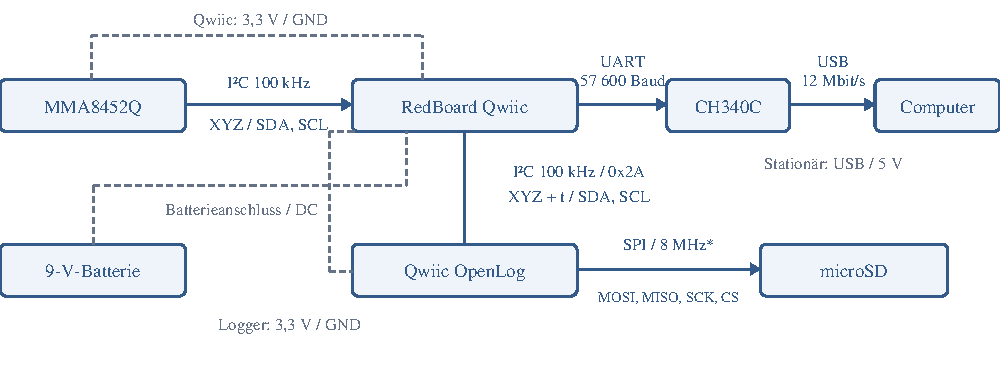
\includegraphics[width=\linewidth]{../ergebnisse/messsystem.pdf}
\caption{Messsystem und Signalpfade. Durchgezogen: Messdaten/Kommunikation;
gestrichelt: Versorgung. Stern: am konkreten Logger noch nicht verifiziert.}
\label{fig:system}\end{figure}
\textbf{MMA8452Q:} Der kapazitive Dreiachsensensor digitalisiert die Beschleunigung
im Sensor und liefert X-, Y- und Z-Rohwerte. Die Werte gelangen über I$^2$C zum Mikrocontroller.

\textbf{RedBoard Qwiic:} Der ATmega328P liest den Sensor aus, erzeugt die
Zeitstempel und formatiert die Daten. Die Qwiic-Schnittstelle stellt 3,3-V-Pegel bereit \cite{redboard}.

\textbf{CH340C und Computer:} Die USB-UART-Brücke überträgt die seriellen Daten
zum Computer \cite{redboard}; der Sketch verwendet 57\,600 Baud (8N1).
Auf dem Computer werden die Daten als Text gespeichert und in Python ausgewertet.

\textbf{Qwiic OpenLog:} Der mobile Logger empfängt Daten über I$^2$C und schreibt
sie auf microSD \cite{openlog}. \texttt{Lab1Code2} verwendet die Standardadresse
\texttt{0x2A} und hängt die Messwerte an \texttt{ACCdata.txt} an.

\textbf{microSD und Batterie:} Die microSD speichert die Messung dauerhaft; ihre
interne Anbindung am Logger erfolgt über SPI. Im mobilen Aufbau versorgt eine
9-V-Batterie das Board über dessen vorgesehenen Versorgungseingang, die Module
erhalten geregelte 3,3 V (gemeinsame Masse).

\textbf{Bustakte:} I$^2$C verwendet den 100-kHz-Standardtakt der Wire-Bibliothek.
Die USB-Brücke arbeitet im Full-Speed-Modus (12 Mbit/s), der UART-Pfad mit
57\,600 bit/s; beides ist von der Abtastfrequenz zu unterscheiden \cite{ch340}.
Die im bisherigen Bericht genannten 8 MHz für SPI sind eine Firmwareannahme,
kein am Laborgerät bestätigter Wert. Dieser Takt bleibt vor Abgabe zu prüfen.
\clearpage

\section{Temperatur und Sensoreinheiten (Aufgaben 2--3)}
\subsection*{Aufgabe 2: Temperatur aus ADC-Code 520}
Angenommen werden eine lineare Sensor-Kennlinie ohne Offset und eine ADC-Referenz
von 5 V. Bei 10 Bit gibt es $2^{10}=1024$ Codes von 0 bis 1023.
Die übliche Endpunkt-Näherung liefert
\begin{align}
U &= \frac{520}{1023}\,5\,\mathrm{V}=2{,}5415\,\mathrm{V},\formeleintragalign{ADC-Code in Spannung umrechnen}\\
T &= \frac{U}{3{,}3\,\mathrm{V}}\,40\,{}^\circ\mathrm{C}
   =\frac{520\cdot5\cdot40}{1023\cdot3{,}3}\,{}^\circ\mathrm{C}
   \approx\boxed{30{,}81\,{}^\circ\mathrm{C}}.\formeleintragalign{Temperatur aus Sensorspannung}
\end{align}
Bei Verwendung der idealen ADC-Schrittweite $5/1024$ V ergibt sich stattdessen
$30{,}78\,{}^\circ$C. Die Differenz von etwa $0{,}03\,{}^\circ$C liegt unter
einem Quantisierungsschritt von etwa $0{,}059\,{}^\circ$C; beide Näherungen sind
bei genannter Konvention konsistent. Die 3,3 V beschreiben hier den
Sensorausgang, nicht die 5-V-ADC-Referenz.

\subsection*{Aufgabe 3: Achsen und physikalische Umrechnung}
Die Sketch-Funktionen \texttt{getX()}, \texttt{getY()} und \texttt{getZ()}
liefern in dieser Reihenfolge vorzeichenbehaftete Rohwerte (Counts), keine
SI-Beschleunigungen \cite{library}. Die Achsenzuordnung wird durch nacheinander
senkrechtes Ausrichten der aufgedruckten positiven und negativen Achsen geprüft:
Die vertikale Achse zeigt näherungsweise $\pm1\,g$, die beiden anderen etwa null.
Die Achsenrichtung ist beim Vergleich von Ober- und Unteransicht zu beachten
(Datenblatt S. 3--4) \cite{mma}.

Die 12-Bit-Werte besitzen 4096 Codes. Aus dem Datenblatt (S. 6) und der
Anwendungsnotiz ergeben sich folgende Umrechnungen \cite{mma,an4076}:
\begin{center}
\begin{tabular}{c|c|c}
Messbereich & Empfindlichkeit $S$ & Umrechnung in $g$\\\hline
$\pm2\,g$ & 1024 Counts/$g$ & $r/1024$\\
$\pm4\,g$ & 512 Counts/$g$ & $r/512$\\
$\pm8\,g$ & 256 Counts/$g$ & $r/256$
\end{tabular}\end{center}
Mit Rohwert $r$ gilt
\begin{equation}
a=(r/S)\cdot9{,}80665\,\mathrm{m/s^2}.
\formeleintrag{Rohwert in Beschleunigung umrechnen}
\end{equation}
Beispielsweise entsprechen 1024 Counts bei $\pm2\,g$ genau
$1\,g=9{,}80665\,\mathrm{m/s^2}$ (mit der verwendeten Normfallbeschleunigung).

\textbf{Dateninterpretation:} Die Dateinamen kennzeichnen $\pm2\,g$ bzw.
$\pm4\,g$; Ruhesignale und der vorhandene Rohwert-Sketch stützen die Interpretation
als Counts. Für die späteren Dateien steht die Zeit jedoch in Spalte 1 statt
Spalte 4. Die historische Firmware ist nicht für jede Aufnahme gesichert:
Sollten die exportierten Werte bereits mg sein, muss deren Einheit vor Abgabe
bestätigt und die Umrechnung geändert werden. Eine Division durch 1000 oder 500
wird deshalb nicht ohne dokumentierte mg-Ausgabe verwendet.
\clearpage

\section{Bewegungsaufnahme mit kleinem Messbereich (Aufgabe 4)}
Die Datei \texttt{ACC\_Data\_Aufgabe1.4\_2g.12.txt} enthält 144 Messwerte mit
11,260 s Dauer. Die relative Zeit beginnt beim ersten gespeicherten Zeitstempel;
Abbildung~\ref{fig:a4} zeigt vier Sekunden aus der Bewegungsphase.
\begin{figure}[H]\centering
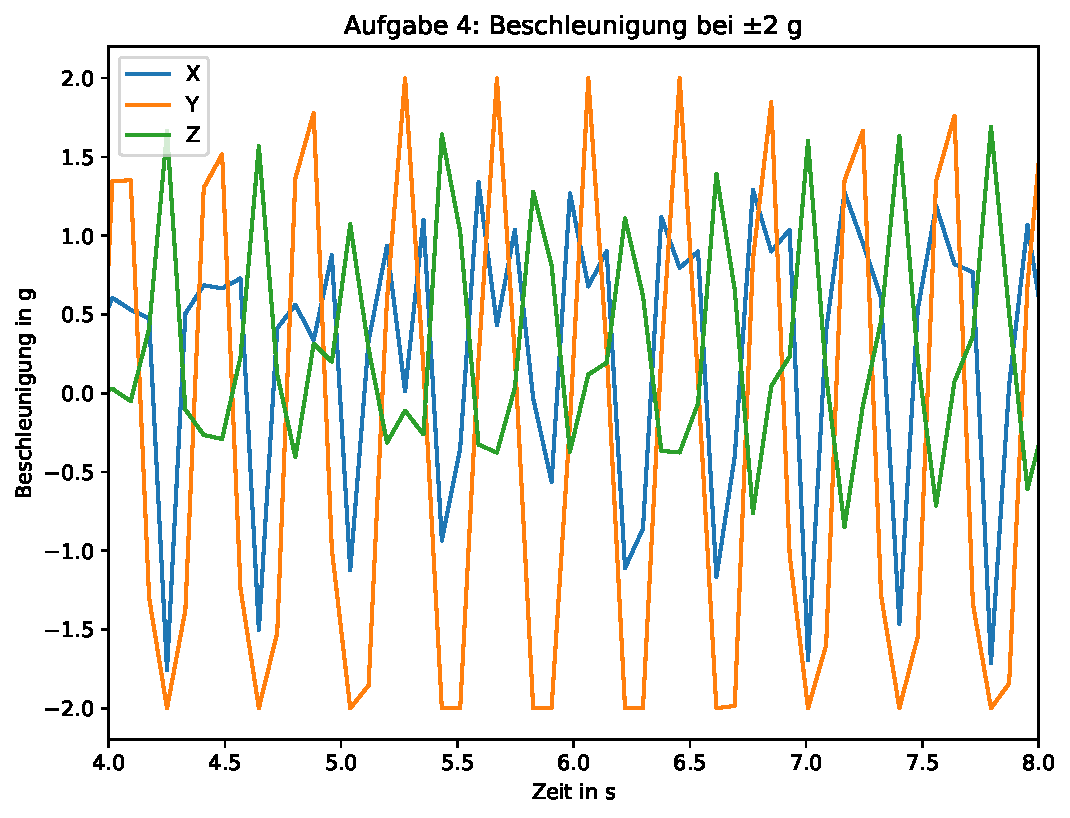
\includegraphics[width=\linewidth]{../ergebnisse/aufgabe4.pdf}
\caption{Aufgabe 4(a): X, Y und Z im Fenster 4--8 s der ursprünglichen Aufnahme.
Die Punkte werden zur Lesbarkeit verbunden; dazwischen liegen keine Messwerte vor.}
\label{fig:a4}\end{figure}

\subsection*{4(b): Plateaus der Peaks}
Die gleich hohen Plateaus entstehen durch Sättigung: Im eingestellten
$\pm2$-$g$-Bereich können größere Beschleunigungen nicht mehr dargestellt
werden. Bei 12 Bit begrenzen die Rohcodes $-2048$ und $+2047$ die Anzeige;
das entspricht $-2\,g$ und etwa $+1{,}999\,g$. Dadurch erscheinen unterschiedlich
starke Spitzen mit gleichem Grenzwert. Die Lösung ist ein größerer Messbereich
($\pm4\,g$ oder bei Bedarf $\pm8\,g$) mit passender Umrechnung; bereits
abgeschnittene Spitzen lassen sich nachträglich nicht rekonstruieren.

\subsection*{4(c): Abweichung von der tatsächlichen Bewegung}
Der Sensor misst Beschleunigung einschließlich der lageabhängigen
Schwerkraftkomponente, nicht die Handposition oder den Weg. Zusätzlich
beschneiden Sättigung und die geringe gespeicherte Rate von rund 12,70 Hz
die Darstellung schneller Vorgänge: Zwischen den Messpunkten liegende Spitzen
können fehlen, und Frequenzanteile oberhalb der Nyquist-Grenze von rund
6,35 Hz können ohne ausreichende Vorfilterung aliasieren. Unbeabsichtigte
Rotation, Sensorauslenkung in der Hand, Offset, Rauschen und Quantisierung
verändern das Signal ebenfalls.

\textbf{Zeitliche Einordnung:} Eine Erhöhung des Messbereichs löst das
Sättigungsproblem, erhöht jedoch nicht automatisch die Zahl gespeicherter
Messpunkte. Diese beiden Ursachen werden in Aufgabe 5 getrennt betrachtet.
\clearpage

\section{Messbereich und Datenrate anpassen (Aufgabe 5)}
\textbf{Messbereich.} Das Register \texttt{XYZ\_DATA\_CFG} (Adresse
\texttt{0x0E}) legt über \texttt{FS[1:0]} den Messbereich fest. Das Datenblatt
(Rev. 10, S. 23) nennt $00$ für $\pm2\,g$, $01$ für $\pm4\,g$ und $10$ für
$\pm8\,g$. $11$ ist reserviert \cite{mma}. Für die Wiederholung setzt
\texttt{Lab1Code1} mit \texttt{SCALE\_4G} den Wert $01$. Dadurch lassen sich
Spitzen jenseits von $\pm2\,g$ erfassen, bei einer feineren Auflösung als im
$\pm8$-$g$-Bereich (512 gegenüber 256 Counts pro $g$).

\textbf{Datenrate.} Zusätzlich setzt \texttt{ODR\_100} im Register
\texttt{CTRL\_REG1} (\texttt{0x2A}) das Feld \texttt{DR[2:0]} auf $011$.
Die Bitwerte $000$ bis $111$ entsprechen 800, 400, 200, 100, 50, 12,5, 6,25
und 1,56 Hz (Datenblatt S. 40--41) \cite{mma,library}.

\begin{figure}[H]\centering
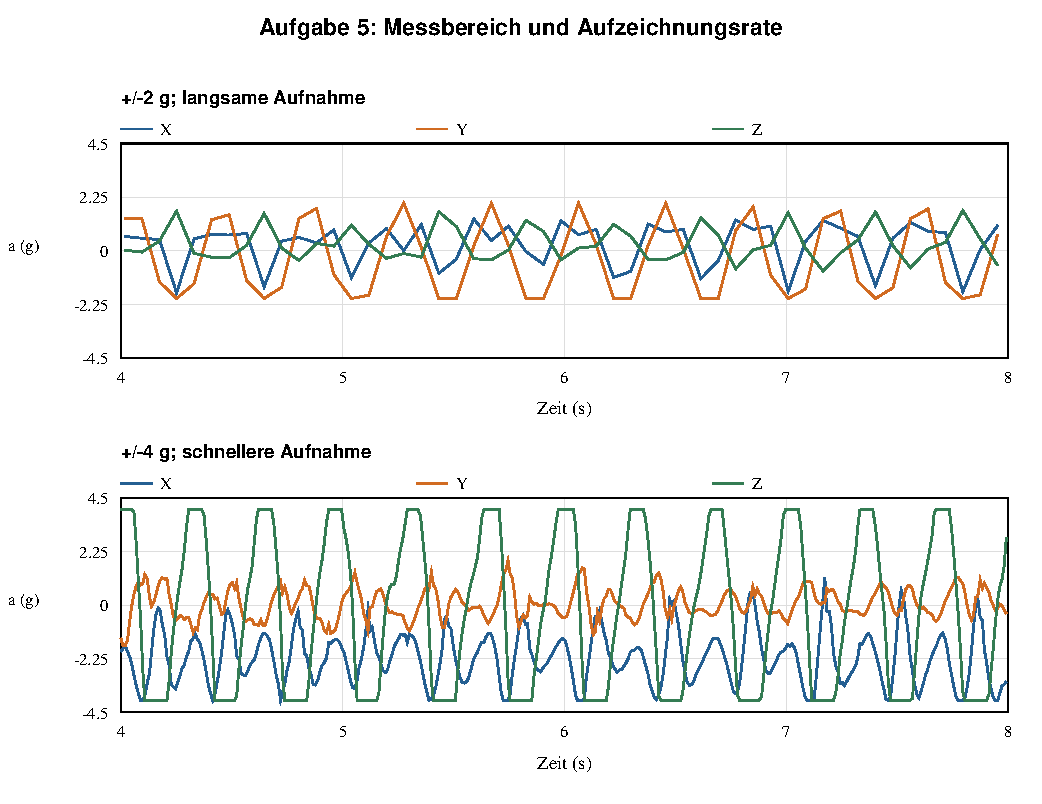
\includegraphics[width=.87\linewidth]{../ergebnisse/aufgabe5.pdf}
\caption[Vergleich der Bewegungsaufnahmen mit $\pm2\,g$ und $\pm4\,g$]{Je
vier Sekunden aus zwei Bewegungsaufnahmen mit gemeinsamer y-Skala.
Oben $\pm2\,g$ bei 12,70 Hz, unten $\pm4\,g$ bei 101,49 Hz gespeicherter Rate.}
\label{fig:a5}\end{figure}

Beide Signale in Abb.~\ref{fig:a5} zeigen wiederkehrende Ausschläge durch die
Handbewegung. Im oberen Plot sind Spitzen an der $\pm2$-$g$-Grenze abgeflacht.
Die Wiederholung erfasst auch Ausschläge über $2\,g$ und zeichnet durch die
höhere Datenrate mehr Messpunkte pro Bewegung auf. Einzelne Spitzen
erreichen weiterhin $-4\,g$. Für solche Bewegungen bietet $\pm8\,g$ mehr
Reserve. Da die Handbewegungen separat ausgeführt wurden und beide
Einstellungen geändert wurden, lassen sich die Verläufe nur qualitativ vergleichen.
\clearpage

\section{Sechs Orientierungen (Aufgabe 6)}
Die Datei \texttt{ACC\_Data\_Aufgabe1.6\_2g.12.txt} enthält 790 Messwerte
in einer durchgehenden Zeitfolge über 62,158 s. Es werden keine getrennten
Abschnitte aneinandergefügt oder Drehphasen aus dem Gesamtplot entfernt.
\begin{figure}[H]\centering
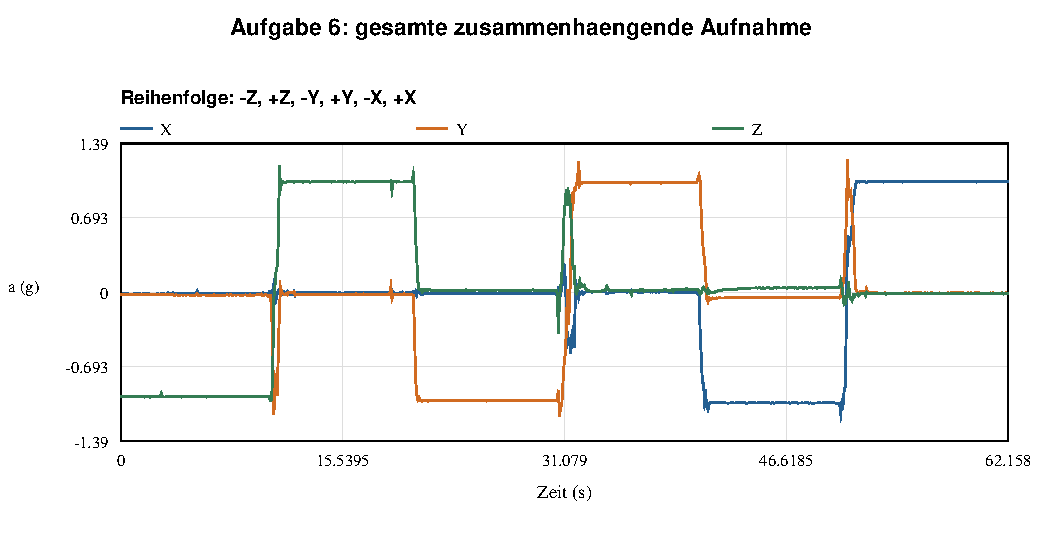
\includegraphics[width=\linewidth]{../ergebnisse/aufgabe6.pdf}
\caption{Gesamte Aufnahme mit den Lagen $-Z,+Z,-Y,+Y,-X,+X$ und allen Übergängen.}
\label{fig:a6}\end{figure}
Zur quantitativen Prüfung werden ruhige Innenfenster ausgewählt. Die
Mittelwerte in Tabelle~\ref{tab:lagen} beruhen auf ungefilterten Daten;
die vollständigen Zahlen und Streuungen stehen in \texttt{orientierungen.csv}.
\begin{table}[H]\centering
\caption{Mittelwerte der ruhigen Innenfenster, relativ zum Aufnahmestart.}
\label{tab:lagen}
\begin{tabular}{c|c|r|r|r}
Lage & Fenster (s) & $\bar a_X$ ($g$) & $\bar a_Y$ ($g$) & $\bar a_Z$ ($g$)\\\hline
$-Z$ & 1--9 & $-0{,}0102$ & $-0{,}0231$ & $-0{,}9700$\\
$+Z$ & 12--19 & $-0{,}0046$ & $-0{,}0174$ & $+1{,}0278$\\
$-Y$ & 22--29 & $-0{,}0116$ & $-1{,}0080$ & $+0{,}0205$\\
$+Y$ & 33--39 & $+0{,}0047$ & $+1{,}0200$ & $+0{,}0178$\\
$-X$ & 42--49 & $-1{,}0284$ & $-0{,}0469$ & $+0{,}0380$\\
$+X$ & 53--61 & $+1{,}0289$ & $-0{,}0063$ & $-0{,}0106$
\end{tabular}\end{table}

\textbf{6(b):} Die Daten sind plausibel: Die jeweilige Hauptachse liegt
näherungsweise bei $\pm1\,g$, die Querachsen nahe null. Die maximale Abweichung
des Hauptachsen-Mittelwerts vom Sollwert beträgt rund $0{,}030\,g$.
Diese Abweichungen lassen sich durch Offset, Empfindlichkeitsfehler und
nicht exakt senkrechte Ausrichtung erklären; die Daten allein trennen diese
Ursachen nicht. Der ruhende Sensor liefert wegen der Stützkraft kein Nullsignal.


\clearpage

\section{Filtervergleich (Aufgabe 7)}
\begin{figure}[H]\centering
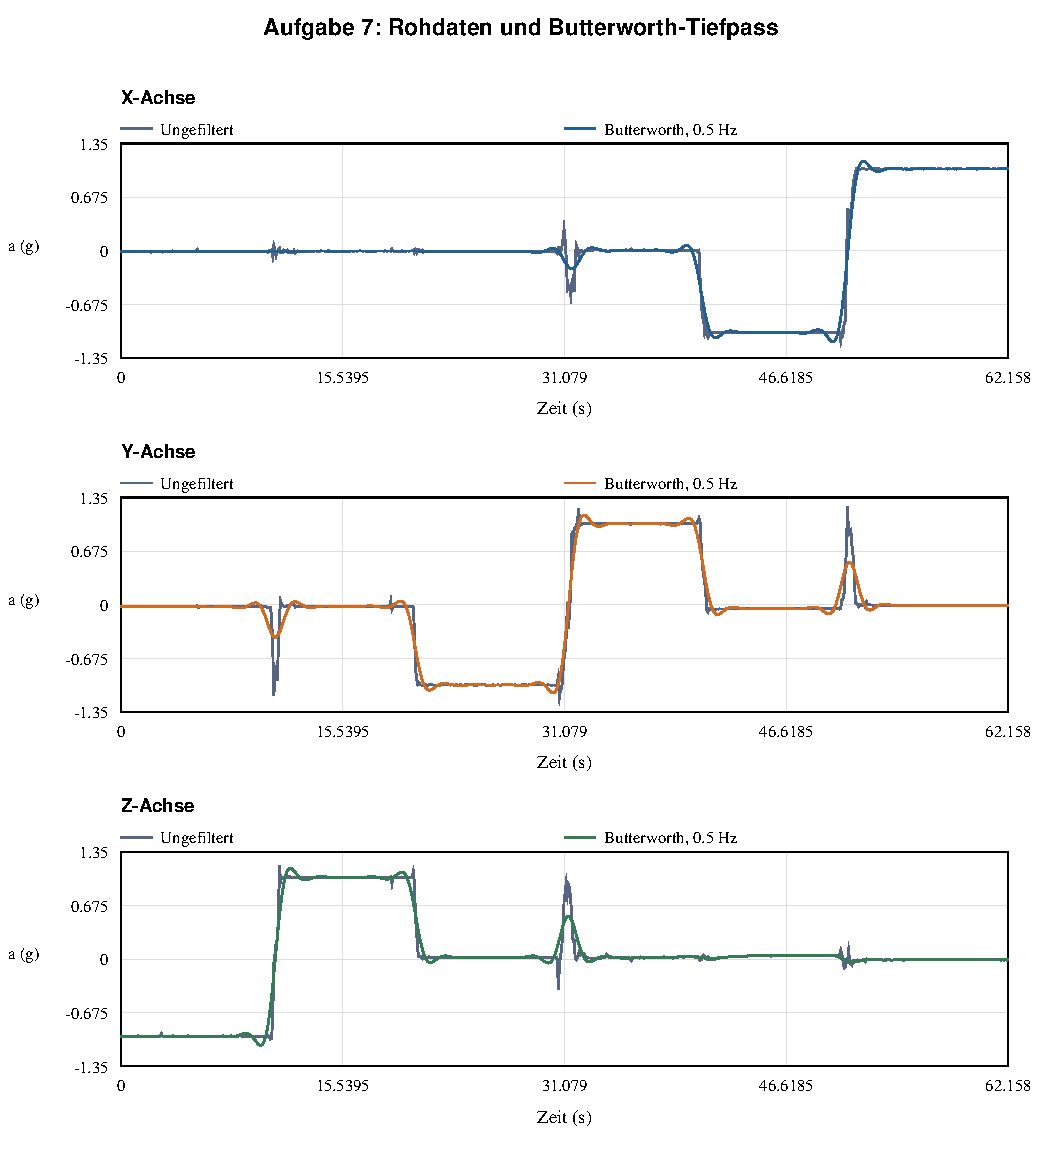
\includegraphics[width=.85\linewidth]{../ergebnisse/aufgabe7.pdf}
\caption{Ungefilterte und gefilterte Beschleunigungen derselben Aufnahme;
jede Achse mit eigener Rohsignal- und Filterkurve.}
\label{fig:a7}\end{figure}

Jede Achse wird mit einem Butterworth-Tiefpass vierter Ordnung und
einer Grenzfrequenz von $0{,}5$ Hz gefiltert. Bezogen auf die effektive
Abtastfrequenz $f_s=12{,}6935$ Hz lautet die normierte Grenzfrequenz
\begin{equation}
W_n = \frac{f_c}{f_s/2} \approx 0{,}0788.
\formeleintrag{Normierte Grenzfrequenz des Butterworth-Tiefpasses}
\end{equation}
Der Filter dämpft schnelle Schwankungen und behält die stationären Lagewerte
bei. Der Vorwärts- und Rückwärtslauf mit \texttt{filtfilt} vermeidet eine
Phasenverschiebung. Dabei wird der Betrag des Frequenzgangs quadriert.
An den Drehübergängen werden auch schnelle Signaländerungen geglättet
(Abb.~\ref{fig:a7}). Die Auswertung der Ruhelagen und der Abtastfrequenz
erfolgt mit den Originaldaten.
\clearpage

\section{Abtastfrequenz und Streuung (Aufgabe 8)}
Die Zeitspalte enthält Millisekundenwerte; der vorhandene Sketch nutzt
\texttt{millis()} auf dem Mikrocontroller. Da der damalige Sketch-Stand nicht
für alle Dateien archiviert ist, bleibt diese Zuordnung eine dokumentierte
Interpretation; Zeitstempel der seriellen Konsole werden nicht verwendet.
Für die 790 Messpunkte ergeben sich 789 Zeitintervalle:
\begin{align}
\Delta t_i&=\frac{t_{i+1,\mathrm{ms}}-t_{i,\mathrm{ms}}}{1000},
& f_i&=\frac{1}{\Delta t_i},\formeleintragalign{Abtastintervall und lokale Frequenz}\\
\bar f&=\frac{1}{789}\sum_{i=1}^{789}f_i,
& s_f&=\sqrt{\frac{1}{788}\sum_{i=1}^{789}(f_i-\bar f)^2}.\formeleintragalign{Mittelwert und Standardabweichung der lokalen Frequenz}
\end{align}
\begin{center}
\begin{tabular}{l|r}
Kennwert & Ergebnis\\\hline
Mittleres Intervall $\overline{\Delta t}$ & 78,7807 ms\\
Standardabweichung $s_{\Delta t}$ & 0,5297 ms\\
Kleinstes / größtes Intervall & 77 / 80 ms\\
Mittelwert der lokalen Frequenzen $\bar f$ & 12,6940 Hz\\
Stichproben-Standardabweichung $s_f$ & 0,0859 Hz\\
Effektive Rate $f_\mathrm{eff}=(N-1)/(t_{N-1}-t_0)$ & 12,6935 Hz
\end{tabular}\end{center}
\begin{figure}[H]\centering
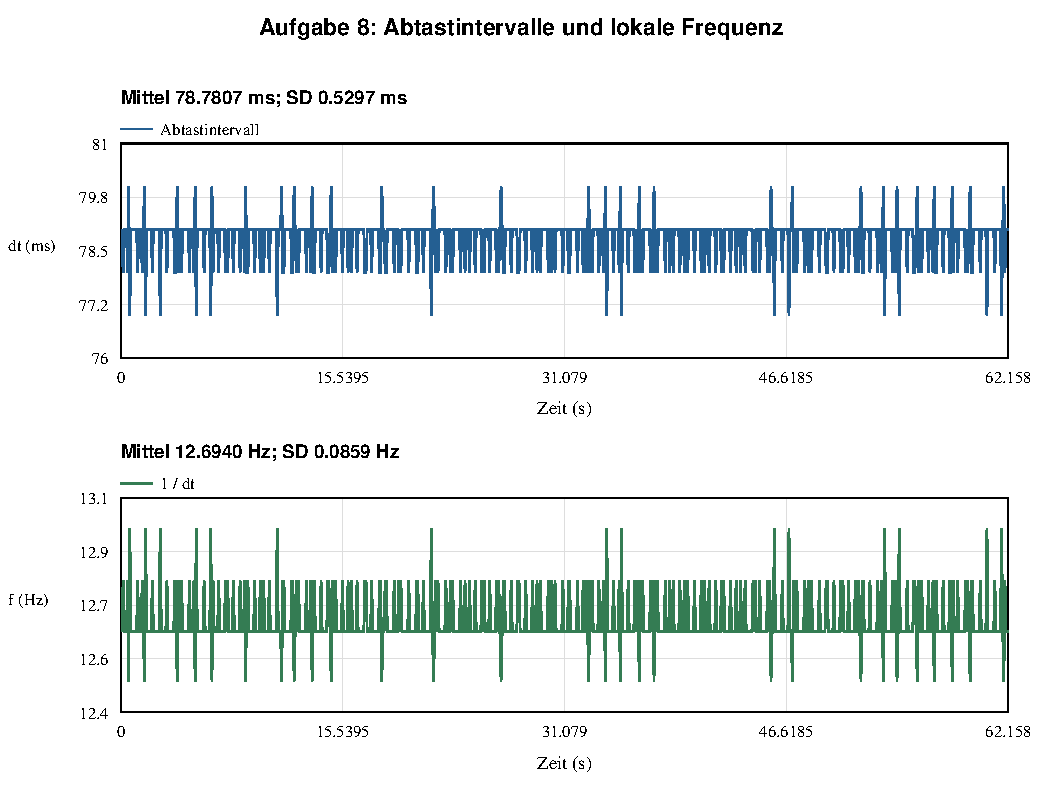
\includegraphics[width=.90\linewidth]{../ergebnisse/aufgabe8.pdf}
\caption{Zeitintervalle und deren Kehrwerte für die vollständige Aufnahme aus
Aufgabe 6. Beide Reihen zeigen dieselbe Zeitinformation in verschiedener Darstellung.}
\label{fig:a8}\end{figure}
Die geringe Differenz zwischen $\bar f$ und $f_\mathrm{eff}$ entsteht durch die
nichtlineare Kehrwertbildung. Die auf 1 ms quantisierten Zeitstempel beeinflussen
die berechnete Streuung; sie ist kein isolierter Messwert des Sensorjitters.
Die gespeicherte Rate ist außerdem von der programmierten Sensor-ODR zu
unterscheiden. Berechnung und Abbildung~\ref{fig:a8} entstehen im Notebook ohne
fest eingetragene Abtastfrequenz.
\clearpage

\section{Mobile Messung und Reproduzierbarkeit (Aufgaben 9--10)}
\subsection*{Aufgabe 9: Mobile Messung}
\texttt{Lab1Code2} setzt $\pm8\,g$ und 200 Hz Sensor-ODR. Die drei
Beschleunigungen sind nach Division durch 256 bereits in $g$ gespeichert.
Die vierte Spalte enthält \texttt{millis()} des Mikrocontrollers. Die Datei
enthält zwei Zeitrücksprünge. Ausgewertet werden die ersten zehn Sekunden
des letzten monotonen Abschnitts ab Datenzeile 405 (536 Messwerte, 9,985 s
zwischen erstem und letztem Messwert). Die Zeitrücksprünge gehen in keine
Intervallberechnung ein.

\begin{center}
\begin{tabular}{l|r|r}
Aufnahme & $\bar f \pm s_f$ (Hz) & $f_\mathrm{eff}$ (Hz)\\\hline
Stationär, Aufgabe 6 & $12{,}694 \pm 0{,}086$ & 12,693\\
Mobil, Aufgabe 9 & $53{,}698 \pm 2{,}468$ & 53,580
\end{tabular}
\end{center}
Die mobile Aufzeichnung liefert häufiger Messwerte und zeigt eine größere
Streuung. Die Sensor-ODR von 200 Hz ermöglicht häufigere neue Messwerte,
doch die mobile Schleife erreicht sie nicht. Pro Zeile führt sie einen
Append-Aufruf, drei separate Sensorabfragen und mehrere I$^2$C-Übertragungen
zum Logger aus. Dieser Aufwand und mögliche SD-Puffer- oder Schreibzeiten
begrenzen die gespeicherte Rate. Die Zeitstempel werden erst nach der
Übertragung der Achsenwerte erfasst. Schwankende Laufzeiten bis zu diesem
Punkt wirken sich auf die gemessenen Intervalle aus. Die einzelnen Einflüsse
lassen sich aus dieser Aufnahme allein nicht quantifizieren.

\subsection*{Aufgabe 10: Ausführbarkeit}
Die Datei \texttt{MainCode1.ipynb} arbeitet die verlangten Aufgaben der Reihe
nach ab. Alle acht Codezellen wurden in einem frischen Python-Prozess
zellenweise ausgeführt; die Auswertung zu 4--9 und die eingebetteten
Abbildungen stammen aus diesem Durchlauf. Geprüft werden streng steigende
Zeitstempel, Rohwertgrenzen, Umrechnung, Filterdimensionen und vorhandene
Plotexporte. Ein interaktiver Jupyter-Kerneldurchlauf und ein Hardwaretest
des neuen Arduino-Sketches wurden hier nicht durchgeführt.

Originaldaten, Hilfsbibliothek \texttt{lab1.py}, Abhängigkeiten und modifizierter
Sketch liegen bei. Alle Pfade sind relativ; die Auswertung benötigt keinen
Netzzugriff. Die Angabe zum SPI-Takt ist im Abschnitt zum Messsystem erläutert.

\begingroup\small
\begin{thebibliography}{9}
\bibitem{mma} NXP, \emph{MMA8452Q, 3-axis, 12-bit/8-bit digital accelerometer},
Rev. 10, 04/2016, S. 3--6, 23, 40--41.
\url{https://www.nxp.com/docs/en/data-sheet/MMA8452Q.pdf}.
\bibitem{an4076} K. Tuck, Freescale/NXP, \emph{AN4076: Data Manipulation and
Basic Settings of the MMA8451, 2, 3Q}, Rev. 1, 02/2012.
\url{https://www.nxp.com/docs/en/application-note/AN4076.pdf}.
\bibitem{library} SparkFun, \emph{SparkFun MMA8452Q Arduino Library},
Quelldatei \texttt{src/SparkFun\_MMA8452Q.cpp}, abgerufen 26.11.2026.
\url{https://github.com/sparkfun/SparkFun_MMA8452Q_Arduino_Library}.
\bibitem{redboard} SparkFun, \emph{RedBoard Qwiic Hookup Guide}, abgerufen 26.11.2026.
\url{https://learn.sparkfun.com/tutorials/redboard-qwiic-hookup-guide}.
\bibitem{openlog} SparkFun, \emph{Qwiic OpenLog}, Hardware/Firmware-Repository,
abgerufen 26.11.2026. \url{https://github.com/sparkfun/Qwiic_OpenLog}.
\bibitem{ch340} WCH, \emph{CH340 Datasheet}, USB Full-Speed serial adapter.
\url{https://www.wch-ic.com/downloads/CH340DS1_PDF.html}.
\end{thebibliography}
\endgroup
\clearpage
\tableofcontents
\addcontentsline{toc}{section}{Abbildungsverzeichnis}
\listoffigures
\addcontentsline{toc}{section}{Formelverzeichnis}
\listofformeln
\end{document}

